\subsubsection{Circular Cylinders}
\noindent
A circular cylinder is what we usually think of as a cylinder.
It is a circle extruded into 3D space.
One of its forms is 
\begin{equation*}
	x^2 + y^2 = R^2,
\end{equation*}
where $R$ is the cylinder's radius.

\begin{figure}[H]
	\centering
	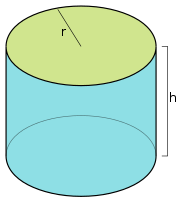
\includegraphics[width=0.33\textwidth]{./differentialMultivariableCalculus/cylinder.png}
	\caption{A circular cylinder}
\end{figure}